\subsection{Random Forests}

A random forest was computed in figure \ref{fig:success_time_vs_trees_randomForest} using G3M2 data as test set and the remaining 15 students as train set.
The number of trees was varied and the time measured.

\begin{figure}[H]
\centering
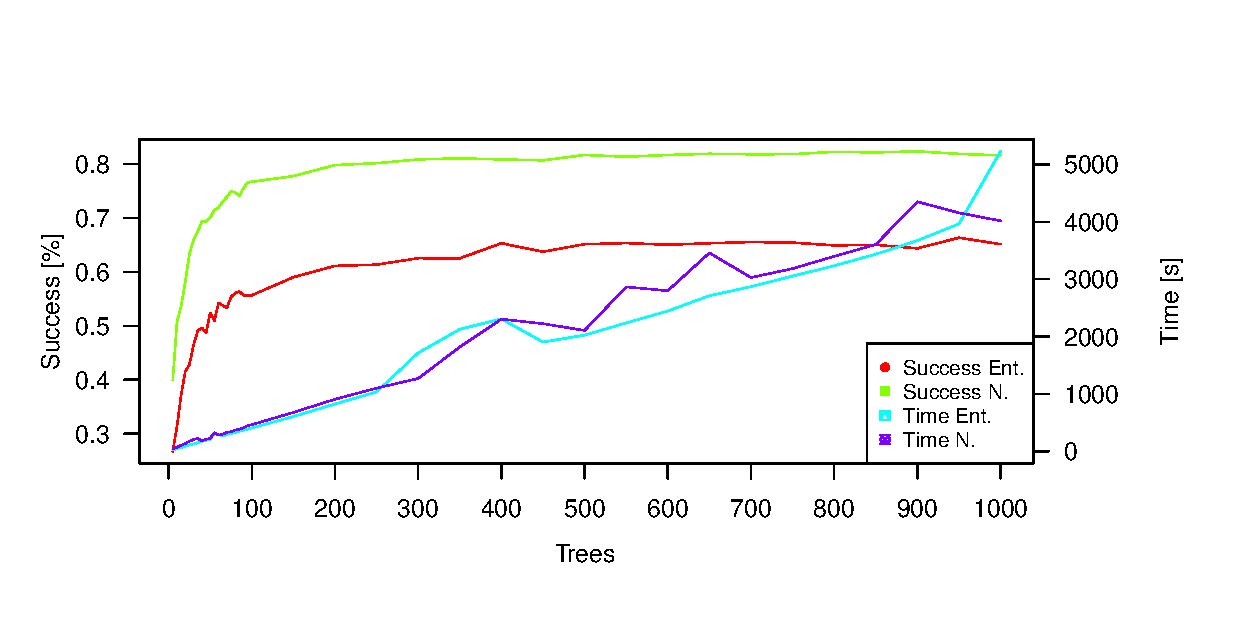
\includegraphics[width = 0.95 \textwidth]{graphics/successRate_randomForest}
\caption{Success rate and time taken to compute the trees needed in the random forest as the number of trees increases.}
\label{fig:success_time_vs_trees_randomForest}
\end{figure}

As can be seen on figure \ref{fig:success_time_vs_trees_randomForest}, then the success rate increases drastically from 0 to 500 trees in the random forest where it settles at around 70\%.
The time increases exponentially with the number of trees.

From figure \ref{fig:success_time_vs_trees_randomForest} it was decided to use 700 trees for the optimum random forest.
Figure ... was generated using the 700 trees.
Each point was computed using 


\Huge{Make comparison of all with best forest settings.}